\documentclass[plainarticle,german,final,hyperref,utf8]{article}
\usepackage{setspace}
\usepackage{listings}
\usepackage{graphicx}
\usepackage{color}

\author{Christian Herold}
\title{SCOREP/GASPI - Tutorial}
 

\definecolor{dkgreen}{rgb}{0,0.6,0}
\definecolor{mauve}{rgb}{0.58,0,0.82}
\definecolor{colorkeyword}{rgb}{0.1,0.1,0.6}
\definecolor{colorassert}{rgb}{0.5,0.5,0.5}


\lstset{
basicstyle=\ttfamily
, frame=single
, numbers=left
, language=C
, numberstyle=\tiny
, stepnumber=1
, showstringspaces=true
, keepspaces=true
, columns=fullflexible
, classoffset=0
, morekeywords={gaspi_rank_t,gaspi_barrier,gaspi_timeout_t,gaspi_return_t,gaspi_config_t,gaspi_proc_init,gaspi_proc_term,gaspi_proc_kill
  ,gaspi_group_commit,gaspi_group_create,gaspi_group_add,gaspi_group_size,gaspi_group_ranks
  ,gaspi_segment_id_t,gaspi_segment_alloc,gaspi_segment_register,gaspi_segment_create
  ,gaspi_segment_ptr,gaspi_queue_id_t,gaspi_offset_t,gaspi_socket_id_t,gaspi_size_t,gaspi_pointer_t
  ,gaspi_write,gaspi_read,gaspi_wait
  ,gaspi_notify,gaspi_notify_reset,gaspi_notify_wait ,gaspi_atomic_value_t
  ,gaspi_proc_num,gaspi_proc_rank
  ,gaspi_number_t,gaspi_notification_t,gaspi_notification_id_t, gaspi_time_t
  ,gaspi_atomic_compare_swap,gaspi_atomic_set
  ,GASPI_SUCCESS,GASPI_TIMEOUT,GASPI_ERROR,GASPI_GROUP_ALL
  ,GASPI_BLOCK,GASPI_TEST,GASPI_CONFIGURATION_DEFAULT,GASPI_NORANK,GASPI_NOSTRING,GASPI_ALLOC_DEFAULT,
  ,gaspi_notify_waitsome,gaspi_notify_size,gaspi_error_message
  ,gaspi_queue_size_max,gaspi_queue_size,gaspi_time_get
  ,gaspi_network_t, gaspi_number_t
  }
, commentstyle=\color{dkgreen}
, keywordstyle=\color{colorkeyword}
, classoffset=1
, morekeywords={ASSERT}
, keywordstyle=\color{colorassert}
, classoffset=0
}

\newcommand{\GASPI}{{\sc Gaspi}}
\newcommand{\SCOREP}{{Score-P}}
\newcommand{\eg}{e.\,g.\ }

\begin{document}

\section*{Build and install \SCOREP{}}

Download and unpack \SCOREP{}. 
Configure it with the {\tt --with-lib} option telling \SCOREP{} where the \GASPI{} and IBVERBS libraries are installed:

\begin{lstlisting}
$ ./configure --with-libGPI2=/home/procs/GPI2-rc2 
              --with-libibverbs15=/home/procs/LibIBverb15
\end{lstlisting}

If the configuration was successful, it prints a summary to the console like this:

\begin{lstlisting}
  Score-P (GASPI backend):

    C99 compiler used:          gcc -std=c99
    libibverbs15 support:       yes, using ...
    libGASPI support:           yes, using ...
    GASPI support:              yes
\end{lstlisting}

Now you can build and install \SCOREP{}:

\begin{lstlisting}
$ make
$ make install
\end{lstlisting}



\section*{Setup \SCOREP{} for instrumenting}

\SCOREP{} is controlled by several environment variables. 
Please refer to the manual of your batch system to ensure, that the environment variables are seen on each node.
Two environment variables are neccessary:

\begin{lstlisting}
$ export SCOREP_ENABLE_TRACING=true
$ export SCOREP_EXPERIMENT_DIRECTORY=/path/to/experiment
\end{lstlisting}

{\tt SCOREP\_ENABLE\_TRACING} activates the tracing.
{\tt SCOREP\_EXPERIMENT\_DIRECTORY} defines the experiment directory, where the traces of your application will be stored.
There are more variables to configure \SCOREP{}, please take look at the manual. 
For instance you can add performance counters with

\begin{lstlisting}
$ export SCOREP_METRIC_PAPI=PAPI_FP_OPS,PAPI_L2_TCM
\end{lstlisting}



\section*{Instrument, compile and execute your application}

Now you can compile and instrument your \GASPI{} application. 

\begin{lstlisting}
./path/to/scorep/bin/scorep --gaspi gcc ./helloworld.c 
                            -o ./helloworld_scorep
\end{lstlisting}

\SCOREP{} will build an instrumented version of your \GASPI{} application, which you can then run like the native version using {\tt gaspi\_run}:

\begin{lstlisting}
gaspi_run -m ./machinefile -n 4 ./helloworld_scorep
\end{lstlisting}

After the application run has finished you can find the traces in the specified experiment directory.
You can use these traces to \eg{} visualize the application run using Vampir.
\begin{figure}[hb]
\centering
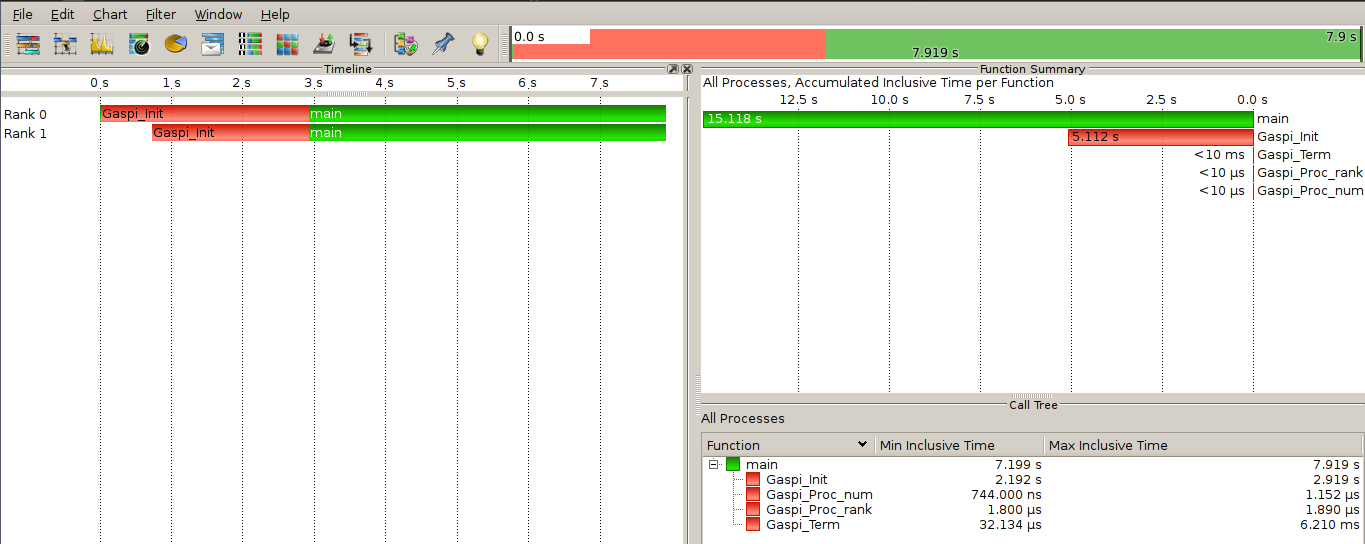
\includegraphics[width=\textwidth]{./trace_all.png}
\caption{Vampir performance visualization}
\end{figure}
\end{document}
